%\section{Antecedentes}
\begin{frame}
	\frametitle{Antecedentes}
	\textbf{ULISES}
	
	\begin{itemize}
		\item Ense\~nar a alumnos habilidades
		\item Unir un sistema interactivo a uno educativo
		\item En definitiva, evaluar
	\end{itemize}
\end{frame}

%\section{Funcionamiento actual}

\begin{frame}
	\frametitle{Antecedentes}
	\framesubtitle{Funcionamiento actual: Nivel de observaci\'on}
	
	\begin{columns}[T] % contents are top vertically aligned
		\begin{column}[T]{5cm} % each column can also be its own environment
			\begin{itemize}
				\item Captura de datos
				\item Se crean
				\begin{itemize}
					\item Propiedades
					\item Observaciones
				\end{itemize}
			\end{itemize}
		\end{column}
		\begin{column}[T]{5cm} % alternative top-align that's better for 
		%graphics
			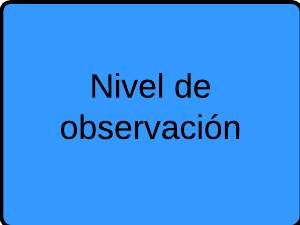
\includegraphics[width=0.5\linewidth]{./Figures/NivelDeObservacion.png}
		\end{column}
	\end{columns}
\end{frame}


\begin{frame}
	\frametitle{Antecedentes}
	\framesubtitle{Funcionamiento actual: Nivel de interpretaci\'on}
	
	\begin{columns}[T] % contents are top vertically aligned
		\begin{column}[T]{5cm} % each column can also be its own environment
			\begin{itemize}
				\item Relaciones entre observaciones
				\begin{itemize}
					\item Pasos
					\item Situaciones
				\end{itemize}
			\end{itemize}
		\end{column}
		\begin{column}[T]{5cm} % alternative top-align that's better for 
			%graphics
			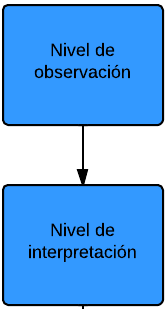
\includegraphics[width=0.5\linewidth]{./Figures/NivelDeInterpretacion.png}
		\end{column}
	\end{columns}
\end{frame}

\begin{frame}
	\frametitle{Antecedentes}
	\framesubtitle{Funcionamiento actual: Nivel de di\'agnostico}
	
	\begin{columns}[T] % contents are top vertically aligned
		\begin{column}[T]{5cm} % each column can also be its own environment
			\begin{itemize}
				\item Usando distintos m\'etodos de diagn\'ostico
				\begin{itemize}
					\item \textit{Clustering}
					\item Clasificaci\'on supervisada
					\item ...
				\end{itemize}
			\end{itemize}
		\end{column}
		\begin{column}[T]{5cm} % alternative top-align that's better for 
			%graphics
			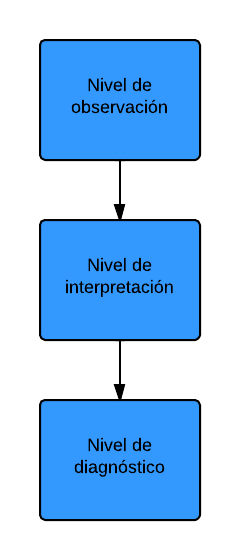
\includegraphics[width=0.5\linewidth]{./Figures/NivelDeDiagnostico.png}
		\end{column}
	\end{columns}
\end{frame}

%\section{Despu\'es del proyecto}
\begin{frame}
	\frametitle{Despu\'es del proyecto}
	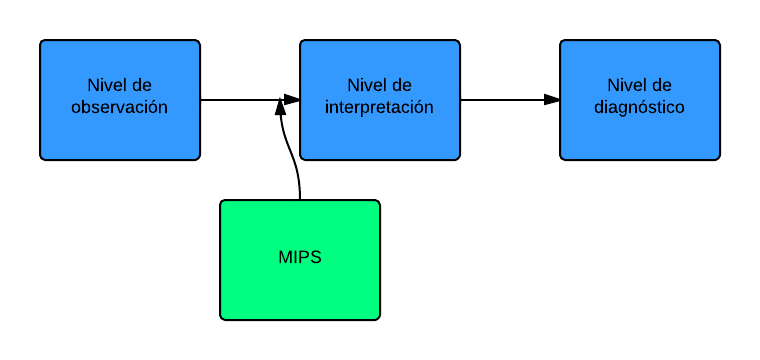
\includegraphics[width=1.0\linewidth]{./Figures/DespuesDelProyecto.png}
	
\end{frame}